\subsection{Methodologies and Experiments}
In this section, we design experimental methodology to rigorously explore the range of possible approaches to dealing with barren plateaus in QNN/VQA development, thus leading to answering the study research question (see Section \ref{Problem Section}).

\subsubsection{Research Context}

\almarginpar{I cannot fit it below, so I include it here: Are the Table 1 elements in any way related to the experimental work? How? Is the number of experiments determined by the cases included in the table? Any relation with Figure 9?}
As explained in the previous section (Section \ref{Literature Review section}), the VQA approach to circuit design for QNN construction overcomes many constraints of the NISQ devices. It allows the construction of trainable circuits, which support development of practical applications in optimisation and machine learning.
However, we have observed the existence of barren plateaus, causing the variance of the cost function gradient to vanish exponentially with the number of qubits.
We have thus investigated three methods to mitigate this phenomenon, i.e. by using a local cost function with shallow circuits, by relying on the identity block and by utilising layerwise learning \cite{cerezoCostFunctionDependent2021, liuParameterInitializationMethod2021, skolikLayerwiseLearningQuantum2021}.

\almarginpar{Provide a reference to the source material for "technology-oriented empirical research". You will need to explain what is such a research, e.g. conducting a series of experiments involving development and study of an IT artefact, I presume - as suggested in the reference you provide}
In the following sections, we will answer the study research question (see Section \ref{Problem Section}) by conducting a series of experiments, with different methods are applied to the same objects, this process is known as \emph{technology-oriented empirical research} \cite{wohlinExperimentationSoftwareEngineering2012}.

We summarise the adopted research process in Figure \ref{Research Activities} and further discuss the first and second phases in section \ref{Research Activities section} 
\almarginpar{You cannot just dump the figure with the research process, you need to explain what is in it, i.e. Figure 9 and the details of its three phases as related to sections 3.1.2 (where is it in the figure?), 3.1.3 (first and second phase), and what happened to the third? You still need to describe it}.

\begin{figure}
    \centering
    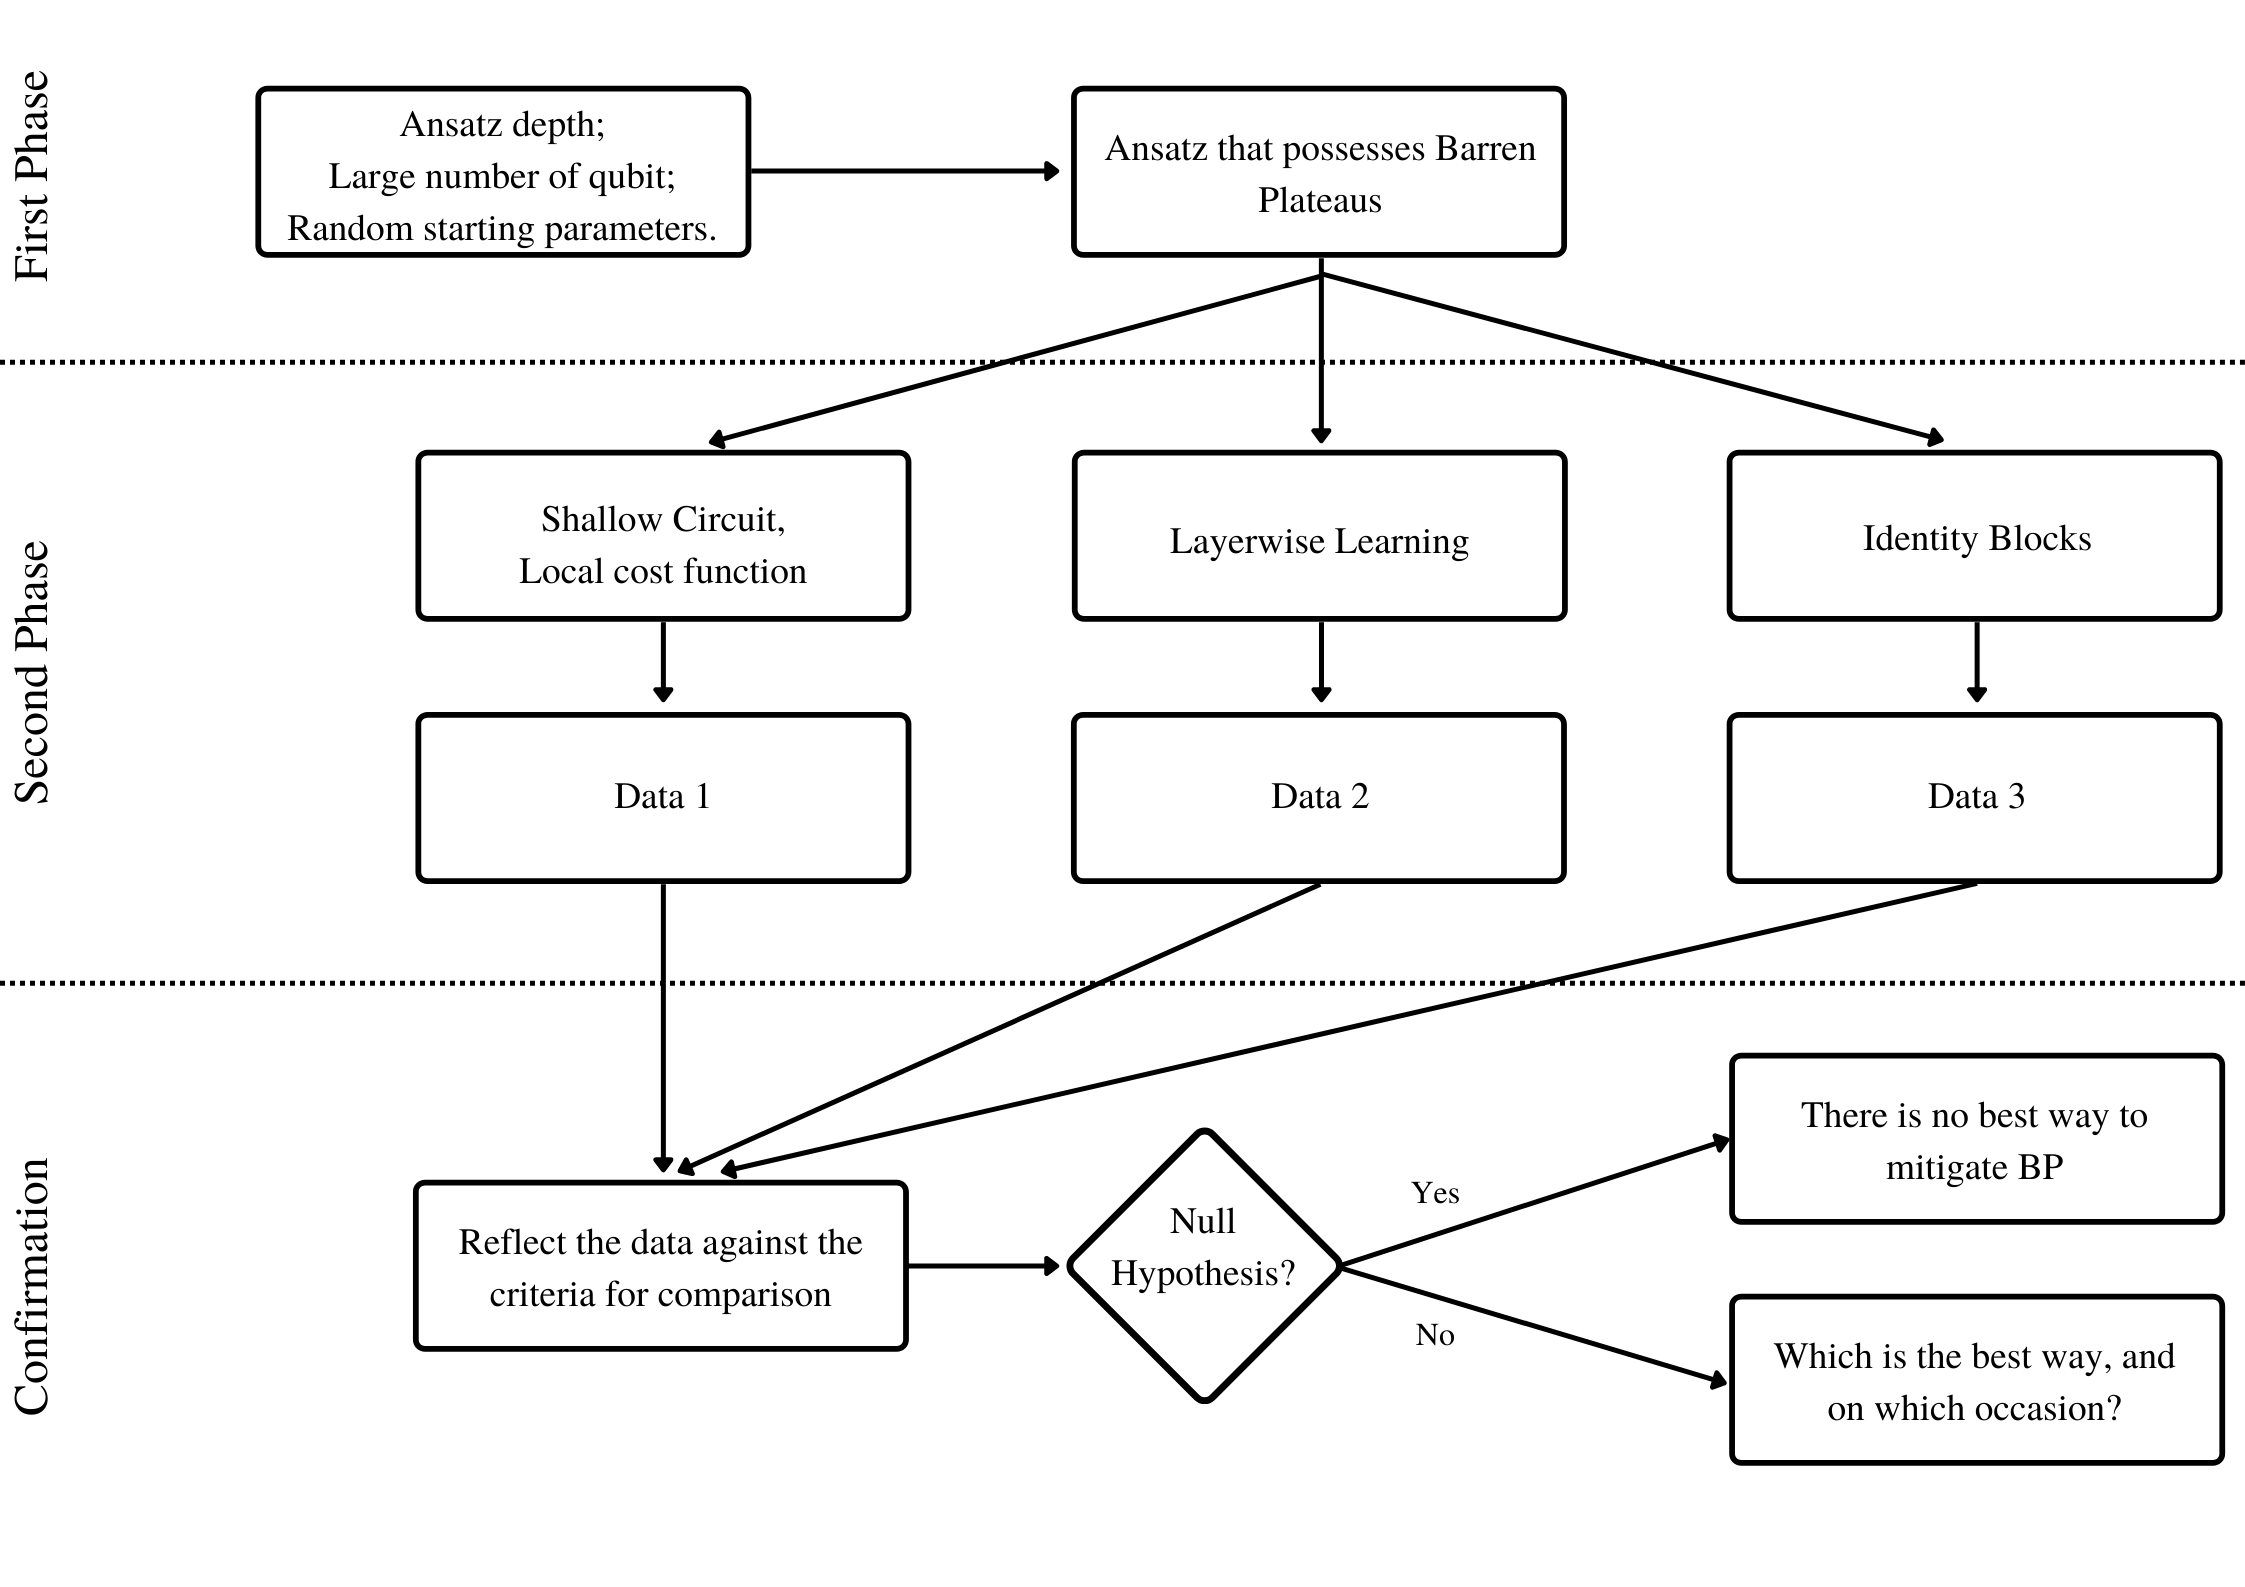
\includegraphics[width=\textwidth]{./ResearchDesign/Appendices/Method.png}
    \caption{
        The adopted research process.
    }
    \label{Research Activities}
\end{figure}

\subsubsection{Objects and Parameters}

As per the context, we can identify the object of study of this research to compare different barren plateaus mitigation methods against different ansatz designs.
One advantage of the empirical experiment is that we can have total control of the experiment environment.
In the context of this research, the parameters that we can vary are:
\begin{itemize}
    \item \textbf{The ansatz designs.} We have chosen the ansatzes NLocal and TwoLocal from Qiskit.
    \item \textbf{The ansatz configuration.} The ansatz object from Qiskit is mutable, which means we can configure their properties to fit the experiment activities. For example, the number of qubits, repetition of layers, and initial parameters.
    \item \textbf{The method to mitigate barren plateaus.} We have reviewed three methods in the literature review, and each of them has configured or trained the ansatz differently.
\end{itemize}

\subsubsection{Research Activities} \label{Research Activities section}
\textbf{In the first phase, we reproduce the barren plateaus phenomenon with the selected ansatzes.}
We can use Qiskit \cite{Qiskit} to construct the ansatzes in a quantum simulator.
The literature review had pointed out that the two factors causing barren plateaus are the \textit{ansatz depth, a large number of qubits} and the \textit{randomised starting parameters}, so we configure the ansatzes to have such characteristics in a quantum simulator.
The optimisation algorithm will be the same in the ansatzes because the main concern is the three methods implemented in the second phase.
\almarginpar{Does it have to shrink "exponentially", what if it shrinks polynomially of high order, is it still good?}We keep track of the variance and the number of qubits to see if the variance is shrinking  \textit{exponentially} (see Figure \ref{Variance Shrinking demo}).
The result of the first phase is the ansatzes that possess barren plateaus.

\almarginpar{So how many experiments will you be running as part of your research activities? From your discussion it is not clear that you will be running any experiments at all!}
\textbf{In the second phase, we implement the three approaches}.
With the QNN ansatzes from the first step, we can implement the three methods discussed in the literature review.
Each of them configures or trains the ansatz differently.
The Qiskit framework also supports the mutation for the ansatz object, such as the number of qubits to measure, the depth of ansatz (repetition) and the starting parameters.
We will track the variances of the gradient for each method to identify if the model has mitigated the barren plateaus phenomenon.
The output is recorded to compare against some criteria (the size of the circuit, execution time, etc.). 
\almarginpar{Where is 6 outcomes coming from? List those outcomes explicitly.}
We expect to have six outcomes.

The results of the research activities are discussed in the Subsection \ref{Data Collecting Section}.

\label{Research Activities section}
\begin{figure}
    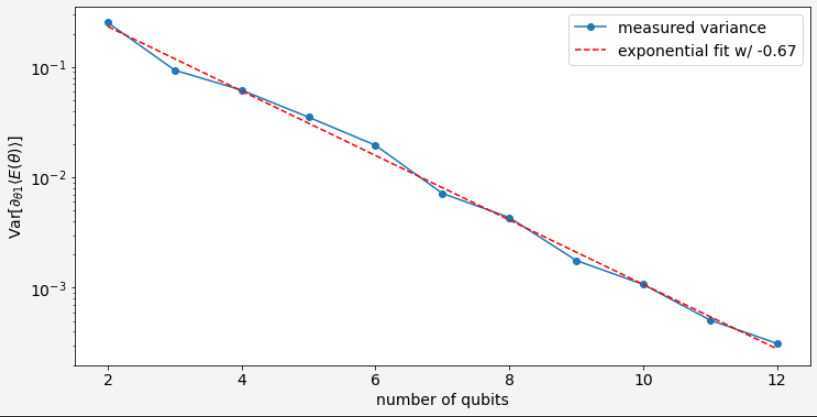
\includegraphics[width=\textwidth]{./ResearchDesign/Appendices/VarianceShrinking.png}
    \caption{
        An example of the barren plateaus phenomenon occurs in a QNN model.
        The variance of the gradient shrinks \textit{exponentially} with the number of qubits.
        Barren plateaus phenomenon prevents optimisation algorithms from navigating the cost function landscape efficiently.
    }
    \label{Variance Shrinking demo}
\end{figure}


\subsubsection{Criteria}
\label{Criteria section}
\almarginpar{I am not sure you provide all these details}We can compare the data with these criteria:
\begin{itemize}
    \item The quality of the solution;
    \item The size of the circuit;
    \item The size of the qubit registry;
    \item The time required to execute the circuit.
\end{itemize}

\subsubsection{Hypothesis}
\almarginpar{I do not think you have done a proper hypothesis testing to claim you have followed the recommended method, you have conducted a qualitative assessment of the experimental work, is this still acceptable according to the adopted methodology - we are missing a reference and a description of this methodology anyway!}The experiment activities are formalised into hypotheses:
\begin{itemize}
    \item \textbf{Null}: The three methods have the same performance according to the criteria, or the difference is insignificant;
    \item \textbf{Alternative}: The three methods' performance differs when reflecting the result against the criteria. If so,
          \begin{itemize}
              \item \textbf{H1}: We can identify which method is the best in specific criteria;
              \item \textbf{H2}: We can recommend the best approach given a context.
          \end{itemize}
\end{itemize}
\almarginpar{I do not think you are planning to do any inferential statistics, and if so what you provided are not really hypotheses, I fail to understand H0, H1 and H2}

\subsubsection{Data Collecting Method}
\label{Data Collecting Section}
\almarginpar{You mention the "expertiments" for the first time? BTW, clearly these are a series of experiments not one experiment!}
Here we discuss our method to collect the data from the \emph{experiments}.

The output of the first phase is Qiskit ansatz objects that contain the number of qubits, the depth of the circuit (rep), and the parameter initialised randomly (refer to the Qiskit document for further detail - *** provide a reference ***).
Moreover, the ansatz object in Qiskit is mutable, which means we can modify the ansatzes properties in the second phase.

For the second phase, we need to record three different outputs of the three methods accordingly, 
\almarginpar{Would this make 9 possible outcomes not 6? Why not 16 according to Table 1?}
with the criteria defined in Subsection \ref{Criteria section}.
The result is a table with the rows of criteria in the Subsection \ref{Criteria section} with each method as rows.
With this data, we can decide whether to reject the null hypothesis or not.

For the null hypothesis case, it means that the methods' performances are relatively the same, and we conclude the experiment.
We will have the result as a table for comparison, which satisfies hypothesis H1.
Then, we need to synthesise the table to answer the research question and verify hypothesis H2.
For example, the method $X$ is the best for the complexity.
\almarginpar{Note that H1 and H2 are not the hypotheses at all! You have clearly listed some objectives to achieve and you are not testing any hypotheses - the research methodology is very poor!}
Finally, we summarise the research results and present the findings.

\subsubsection{Resources}
Most of our required resources are open-sources:
\begin{itemize}
    \item Python 3.6+: \url{https://www.python.org/downloads/}
    \item Jupyter Notebook: \url{https://jupyter.org/}
    \item Qiskit: \url{https://qiskit.org/}
    \item IBM Quantum: \url{https://quantum-computing.ibm.com/}
    \item Qiskit circuit library: \url{https://qiskit.org/documentation/apidoc/circuit_library.html}
\end{itemize}

To prepare the quantum emulator on a local machine, we first install Python and Anaconda for programming language support and Jupyter Notebook as a code editing tool.
Then we follow the official instruction from Qiskit \cite{Qiskit} to install the necessary packages.
We can start working with Qiskit in a Jupyter Notebook file.

\almarginpar{Python "kernel"? do you mean "API"}The other option is to use the provided Python kernel with Qiskit pre-installed provided by IBM Quantum.
While this is a convenient choice for online presentation or remote working because of instant access, this server has shortcomings.
The maximum ram for open access is only 8 Gigabytes, and the processing power is limited.

The quantum emulator from Qiskit is capable of simulating up to 32 qubits.
On the other hand, the actual quantum hardware from IBM is limited to 5 qubits for open access.

\almarginpar{It also offers custom ansatz design, would you explore this option, why not?}Qiskit offers various pre-defined ansatz designs, namely \textit{EfficientSU2, PauliTwoDesign, RealAmplitudes, NLocal}, and \textit{TwoLocal}.
They are popular and frequently studied in quantum chemistry, quantum machine learning, and especially the investigation of barren plateaus.
However, \almarginpar{Not true!}\emph{they are based on the two ansatzes, NLocal and TwoLocal}.
To construct the ansatz as discussed in Section \ref{Research Activities section}, we can use the NLocal and TwoLocal circuits provided.


\subsubsection{Success Condition}
The experiment will be concluded when these conditions are met:
\begin{itemize}
    \item We have QNN ansatzes that can produce barren plateaus;
    \item The three methods are implemented as Python scripts and ready for demonstration;
    \item The data from the three methods are evaluated against the criteria.
\end{itemize}